\section{Special Case Study - MH370}\label{sec:mh370}
The Malaysia Airlines Flight MH370 disappeared on the evening of March the 7th, GMT after losing contact with air traffic control at approximately 5:20pm GMT \cite{Rahman2014}. Publicly available data of the flight after 5:21pm GMT was unavailable, at which point the flight was approximately 6.92$^\circ$N and 101.70$^\circ$E \cite{FlightRadar}. Military radar information suggests that the flight visited a series of known way points west of the planned flight path before being completely lost \cite{ReutersRadar}. Data from satellite pings and international search efforts suggested that the aircraft may have crashed in the Indian Ocean, as illustrated in Figure \ref{fig:mh370_probability_map} \cite{PaulColg, Pandey, ABCNews2014}. As of April 16th 2014, there is an ongoing international effort to attempt to locate the possible crash site and location of the debris from the MH370. 
\begin{figure}[H]
	\centering
	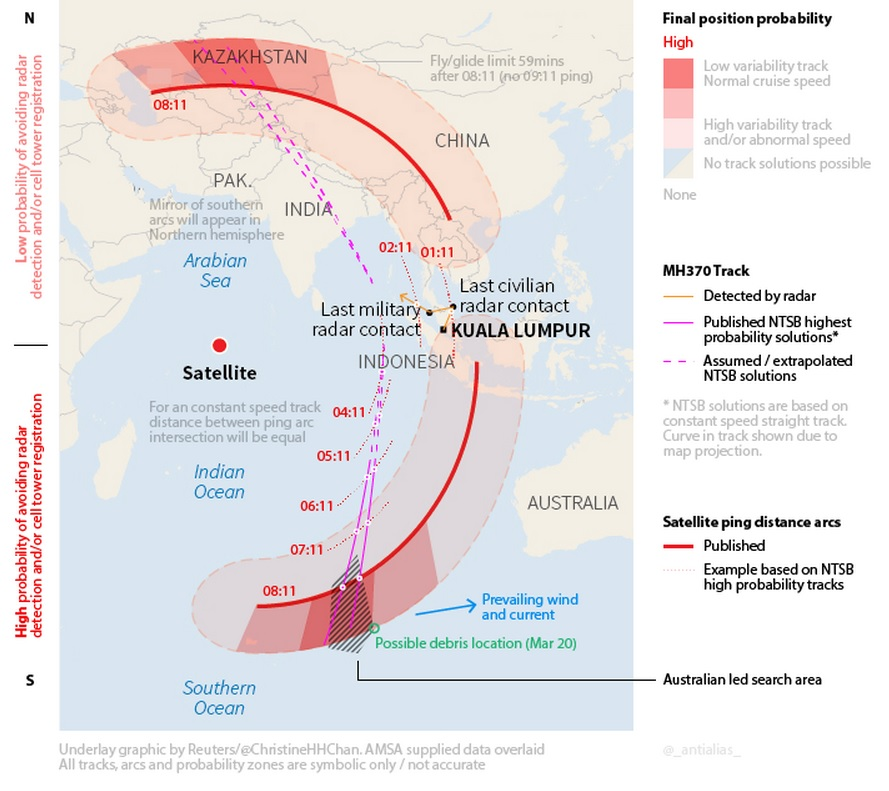
\includegraphics[scale = 0.5]{Pictures/mh370_probability_map.jpg}
	
	\caption[Probability map of possible crash locations of the MH370]{Probability map of possible crash locations of the MH370, reproduced from \cite{PaulColg}}
	\label{fig:mh370_probability_map}
\end{figure}
\subsection{Simulation}
As seen in Figure \ref{fig:mh370_probability_map}, it is most likely that the majority of the flight time after lost radar coverage would be spent over oceanic regions where an ADS-B constellation could provide coverage. The best performing constellation (18 satellites at 700km altitude) was tested against an estimated flight path for the MH370 alongside its standard path. This estimated path assumed that the flight terminated over the Indian Ocean, as shown in Figure \ref{fig:mh370_tot}. For the sake of coverage analysis it was assumed that the ADS-B transponder remained operational for the duration of the flight.
\begin{figure}[H]
	\centering
	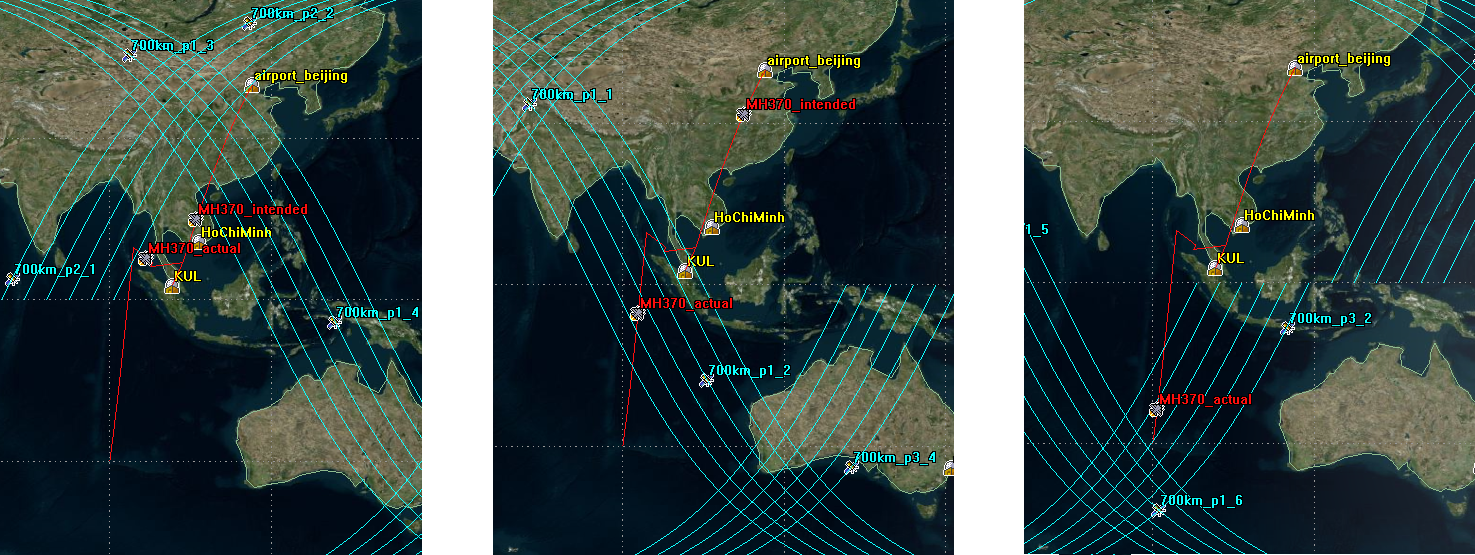
\includegraphics[scale = 0.45]{Pictures/mh370_tot.png}
	
	\caption{Simulated MH370 flight path with 18 satellite constellation}
	\label{fig:mh370_tot}
\end{figure}
\subsection{Results}
The coverage results are summarised in Table \ref{tab:mh370_results}. Results showed that the 18 satellite constellation would have allowed for near constant coverage, with the flight only being out of sight for 10\% of the flight. The high number of discrete accesses for the one flight would have also allowed for deviations in the flight path to be detected early and accurately mapped with many sample points.
\begin{table}[htbp]
  \centering
  \caption{Results from MH370 simulation using 18 satellites}
    \begin{tabular}{lr}
    \toprule
    Parameter & Value \\
    \midrule
    Coverage Gap Fraction & 0.10\% \\
    Discrete Accesses & 20.00 \\
    Maximum Gap & 309.72 seconds \\
    Minimum RX Power & -139.95 dBW \\
    \bottomrule
    \end{tabular}%
  \label{tab:mh370_results}%
\end{table}%
\subsection{Discussion}
The results from this simulation show that the 18 satellite constellation would have provided coverage to almost continually track the MH370 during its flight. If the ADS-B transponder remained operational during the flight, the probable crash and debris locations could be much smaller providing for a much more feasible search area.

The exact status of the ADS-B transponder during the flight is currently unknown. No ADS-B data exists beyond of that reported by \cite{FlightRadar}. ADS-B receivers in the vicinity of this disappearance suggest that the ADS-B transponder was inoperable after this period. In this case the constellation would have not been able to track the entirety of the deviated flight path. However, the high effective ADS-B sample rate of the 18 satellite constellation would have provided a more accurate estimation as to the exact time and location when the ADS-B signal would have been lost. This could have aided in search efforts and generated potential flight paths with greater confidence.
